\begin{figure}[t]
   \centering
   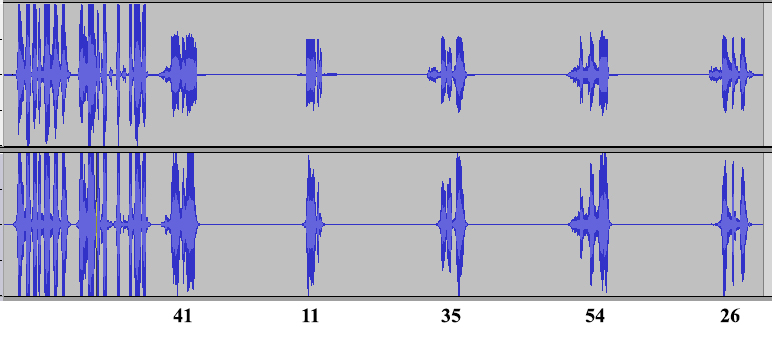
\includegraphics[width=\columnwidth]{figures/Apple1.jpg}.
   \caption{Waveforms of Apple's CAPTCHA, before and after processing, representing "41 11 35 54 26".}
   \label{fig:apple1}
\end{figure}
\begin{figure}[t]
   \centering
   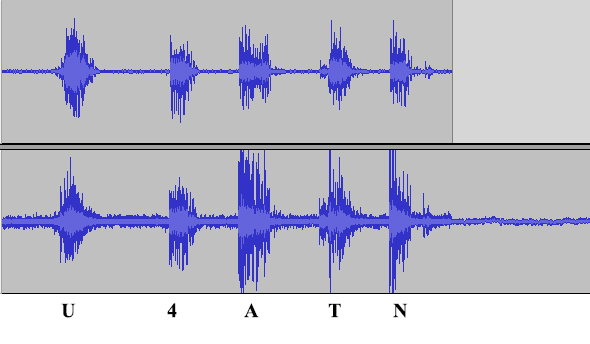
\includegraphics[width=\columnwidth]{figures/BotDetect1.jpg}.
   \caption{Waveforms of BotDetect's CAPTCHA, before and after processing, representing "U4ATN".}
   \label{fig:botdetect1}
\end{figure}

\section{Analysis of audio CAPTCHA systems}
\label{sec:analysis}

This section describes the 8 audio CAPTCHA systems that we analyzed in our previous work, the properties and kinds of noise that make it less discernible to speech recognition services and our approach to overcome those challenges to achieve better accuracy. The results of these experiments are given in Section 8. \newline 

For each CAPTCHA system, the sequence of audio processing techniques, referred to as Action Chains by Audacity, was obtained on a trial-and-error basis with a huge number of CAPTCHAs before the experimental evaluation. We selected cut-off frequency values, amplification factors and filter ranges using spectrum plots of audio samples from each CAPTCHA system.\newline

\subsection{Apple}
\label{sec:apple}

Apple uses its own CAPTCHA system for authenticating humans during apple ID creation. The audio challenge has a male voice spelling out two-digit numbers (from 11 to 99) at equal time intervals. The length of the challenge randomly varies between three to five such numbers. With each number that is spelled out, there is a background noise that makes distinguishing between numbers like fifty-two and sixty-two difficult even for humans. The nature of the noise is external and is composed of sounds of children laughing and talking. There is also a very small internal noise throughout the audio, but we observed that it did not do much to disrupt the speech recognition. The system does not give any margin of errors to users.\newline

The waveforms of Apple's audio CAPTCHA, (representing the challenge "41 11 35 54 26") before and after denoising are shown in Figure 3. To denoise the audio, we equalized the audio using Audacity's standard equalizer with a -18dB bass cut and  +6dB treble boost. We then passed it through a noise gate and low-pass filter to block frequencies higher than 3000Hz and -18dB and frequencies lesser than 500Hz, based on analysis from the spectrum plots. In the resulting audio, we applied noise reduction with a noise profile created for Apple's audio captcha in particular and finally the cleaned up audio was amplified and mixed with a 0.5dB pink noise signal. \newline

\begin{figure}[t]
   \centering
   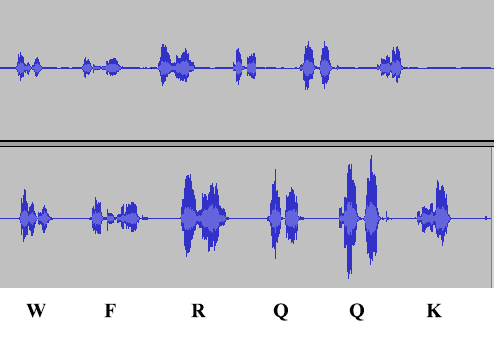
\includegraphics[width=\columnwidth]{figures/captchasnet1.jpg}.
   \caption{Waveforms of captcha.net's CAPTCHA, before and after processing, representing "WFRQQK".}
   \label{fig:captchasnet1}
\end{figure}

\begin{figure}[t]
   \centering
   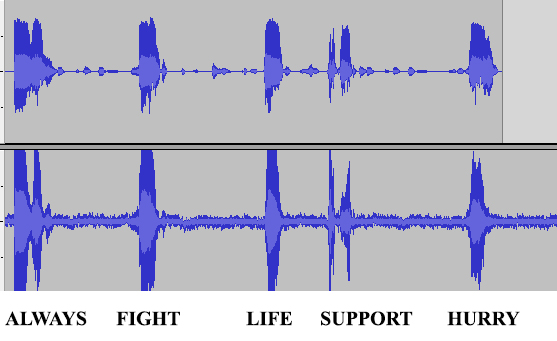
\includegraphics[width=\columnwidth]{figures/Live1.jpg}.
   \caption{Waveforms of Microsoft's CAPTCHA, before and after processing, representing "always fight life support hurry".}
   \label{fig:live1}
\end{figure}


\subsection{BotDetect}
\label{sec:botdetect}

BotDetect is a CAPTCHA system commonly found in several US government websites like the U.S Department of State, Supreme Court of United States, etc. as well as sites like Morgan Stanley, Dell and Intuit. The audio challenge consists of a single male voice spelling out 6 random character that includes alphabets and numbers. It is an open-source CAPTCHA system that allows developers wanting to incorporate BotDetect's CAPTCHA to their websites to play around with the length of the challenge and the kind of noise used in the background. The standard length of challenges is 4-6 characters and the kinds of noises randomly generated in the background include industrial noises, radio, pulse, hive, robot, workshop and others. The system does not have any margin for errors.\newline

To denoise such a CAPTCHA system with dynamically generated background noises was a real challenge. We created a general rule that best worked for many of these noise types, if not all. We filtered the audio file using a high-pass filter to cut off frequencies below 1000Hz, equalized it using the standard values that work best for human speech, amplified by +4dB. Finally, we found that reducing the pitch of the speaker by one scale down (-5.6\%) helped the speech recognizers in better identifying the words.

\subsection{captchas.net}
\label{sec:captchasnet}
Captchas.net is also an open-source CAPTCHA system that is integrated in CMS tools like Joomla and Plone and popular blogs to prevent spam activity. The audio challenge consists of 6 unequally-spaced words spelled with the NATO phonetic alphabets. Users are expected to enter the first alphabet of each of the NATO phonetic words that they hear. For example, the challenge "WFRQQK" in Figure 5 gets spelled out as "Whiskey Foxtrot Romeo Quebec Quebec Kilo" and the user is expected to recognize these words and input "WFRQQK" in the text box given. There is no external background noise that is added. But the voice seems to be robotic and words are of different intensities and pitches which makes it difficult for speech recognition systems to work. This system too requires users to get all 6 characters right.\newline

In an attempt to help speech recognition services to get past the variable space intervals issue, we reduced the tempo of the audio by 20\% and then amplified it by a ratio of 2.26. We then normalized the audio file by a factor of -2.0 to amplify bigger signals and soften the smaller ones. We then truncated the silence caused by reducing the tempo and mixed it with a small pink noise of 0.8dB to get a cleaner version of the audio.\newline

\subsection{Microsoft Live}
\label{sec:live}
Microsoft uses a self-designed CAPTCHA system in its account creation page. The audio challenge consists of random English words v, varying in length (5-7 words), pronounced by a man and a woman, some of which are not perceivable even to humans. Since the words are not from a specific corpora of words, users find it difficult to identify words and often have to make hard choices between words like "quiet" and "quite", and "sure" and "shore". The audio also has a very unique kind of external noise with a female noise speaking in a language different from English in the background. The system expects users to get all the words right.An example of Microsoft's CAPTCHA is shown in Figure 6.\newline

To denoise this kind of CAPTCHA, we equalized the audio with -18dB bass cut and +8dB treble boost and then passed it through a noise gate to ward off signals higher than Hz frequency. We sampled a piece of the background noise and using this as a noise profile, ran a noise reduction algorithm and equalized it again. To mask the noise that was left over, we added a strong pink noise of 0.15dB, higher than the value we used for other systems. This gave us a much cleaner sounding audio with the background noise masked by a clean pink noise. The comparison between the clean and the denoised audio signals can be seen in the image.\newline

\subsection{Google's reCAPTCHA v1 (Dec 2014 version)}
\label{sec:recaptchav1}
Google introduced reCAPTCHA with the title "Stop Spam. Read books." in the year 2011 and over the years kept improving their CAPTCHA system for reasons of usability as well as security. The kind of audio CAPTCHAs that Google used also kept changing. We tested the audio challenge that was present in reCAPTCHA v1(Dec 2014). This version of audio reCAPTCHA had 9-10 digits spoken out by different voices in different accents, all unequally spaced. Some digits had some background noise associated with them and the noise was hissy and internal in nature. It also allowed upto one wrong digit by the user.\newline

We couldn't do much to denoise the reCAPTCHA audio files as techniques like Noise reduction and noise gating further decreased the accuracy of the speech recognition services. So we did a simple slowdown of the audio by reducing the tempo by -25\% and then amplifying the intensity of the sound by a ratio of almost  3.0.\newline

\subsection{Google's reCAPTCHA v2 (Jan 2017 version)}
\label{sec:recaptchav2}
The version 2 of Google's reCAPTCHA was much simpler than its predecessor. It had just 5 digits, spelled out in equal intervals with little to no noise at all. We had a very high accuracy of 98.3\% using Google's Speech API, even before denoising. The system also allowed upto 2 incorrect digits by the user. Since there was little to no noise in the audio files, we did an amplification of the audio followed by reduction in tempo and then equalization.\newline

\subsection{Securimage}
\label{sec:securimage}
Securimage is a free open-source CAPTCHA service that is readily available for integration in PHP. It is being used in many government websites and portals, since it is free and open-source. The CAPTCHA challenge consists of 6 characters with alphabets and digits. The audio has a lot of noise and inconsistent intervals between the characters spelled out. The kinds of noise vary from airport noises, crowds talking, children playing and laughing, industrial noises, musical instruments etc. The amplitude of the noise is so high that sometimes the CAPTCHA's audio gets lost within the noise. This system too does not have any margin for error and expects users to get all 6 characters right.\newline

To clean these audio files, we created a noise profile with all the open-source noise files that Securimage offers and then did a -18dB noise reduction, a reduction in tempo by -20\% and then amplified the signals to make them louder. But the combination of noise files used for each CAPTCHA varied so widely that a general noise profile did not work very well for all captcha challenges.\newline

\subsection{Telerik}
\label{sec:telerik}
Telerik is a company that offers software solutions for web, mobile and desktop application development. Their CMS Sitefinity has many customers including several colleges in University of Illinois. Telerik offers its own CAPTCHA system with an audio alternative. The challenge has a female voice speaking out 5 words that may be NATO words or numbers. The words are spaced at fairly equal intervals, but the tempo at which each word is spoken varies. The nature of the noise is internal with words getting slightly cut and distorted at times.\newline

The noise reduction profile for Telerik consists of an equalization step with a -18dB bass cut and a +8dB treble boost, followed by an amplification and noise gating to gate only frequencies above 1400Hz. The resulting signal is then passed through a low-pass filter to remove frequencies lesser than 300Hz and then slowed down the audio by -20\%. Finally the signal is normalized by -2dB and this resulted in very clean version of the audio that performed better with speech recognition services.





